\documentclass{beamer}
\usepackage[en]{zafu}
% Charts on slides
\usepackage{pgfplots}
\usetikzlibrary{positioning, arrows.meta}
\pgfplotsset{compat=1.17}
% Rules for tables

\usepackage{booktabs}
% Slightly smaller author & affiliation on the title page
\setbeamerfont{author}{size=\small}
\setbeamerfont{institute}{size=\footnotesize}
\setbeamerfont{date}{size=\footnotesize}

% PDF metadata and safe bookmark settings (no visual changes)
\hypersetup{
  pdftitle={A Physics-Informed Synthetic Data Generation Framework for Spectroscopic Analysis},
  pdfauthor={Birrul Walidain; Nasrullah Idris; Khairun Saddami; Natasya Yuzza; Rara Mitaphonna},
  pdfsubject={LIBS; Physics-Informed Synthetic Data; Informer; Calibration-Free Analysis},
  pdfkeywords={LIBS, Synthetic Data, Physics-Informed, Informer, Calibration-Free, Spectroscopy}
}
% Avoid warnings from superscripts and line breaks in PDF strings
\pdfstringdefDisableCommands{%%
  \def\\{}%% ignore manual line breaks in bookmarks
  \def\textsuperscript#1{#1}%% drop superscript styling in bookmarks
}

\title[Physics-Informed Synthetic Data for Calibration-Free LIBS]{A Physics-Informed Synthetic Data Generation Framework for Spectroscopic Analysis}
\subtitle{Case Study: Traditional Women’s Medicine Sold in Banda Aceh}
\author[Walidain et al.]{
  Birrul Walidain\textsuperscript{1,2},
  Nasrullah Idris\textsuperscript{1*},\\
  Khairun Saddami\textsuperscript{3},
  Natasya Yuzza\textsuperscript{1,2},
  Rara Mitaphonna\textsuperscript{4}
}
\institute{
  \footnotesize
  \textsuperscript{1}Department of Physics, Faculty of Mathematics and Natural Sciences, Universitas Syiah Kuala, Banda Aceh 23111, Indonesia\\
  \textsuperscript{2}Graduate School of Mathematics and Applied Sciences, Universitas Syiah Kuala, Banda Aceh 23111, Indonesia\\
  \textsuperscript{3}Department of Electrical and Computer Engineering, Universitas Syiah Kuala, Banda Aceh 23111, Indonesia\\
  \textsuperscript{4}Research Center for Photonics, National Research and Innovation Agency (BRIN), South Tangerang 15314, Indonesia\\
  \vspace{0.5em}
  \textsuperscript{*}Corresponding author: \texttt{nasrullah.idris@usk.ac.id}
}
\date{September 5, 2025}

% Optional: small logo on title (uses your USK logo)
\titlegraphic{\includegraphics[width=0.16\textwidth]{src/logo-usk.png}}

\begin{document}

% Slide 1: Title Slide (0:00–0:30)
\maketitle

% --- Combined: Empowerment Promise + Purpose (Visual 4 Boxes) ---
\begin{frame}{Promise \& Purpose}
  \textbf{In the next 10 minutes, you will learn how to:}
  \vspace{0.8em}

  \begin{center}
  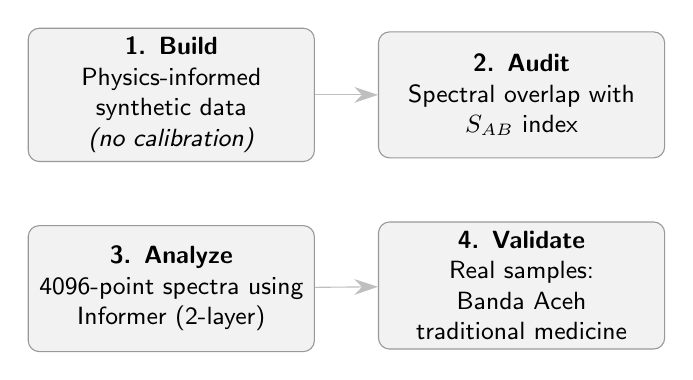
\begin{tikzpicture}[node distance=0.8cm and 0.8cm]
    \tikzset{
      box/.style={
        rectangle, rounded corners,
        draw=black!40, fill=gray!10,
        text width=3.4cm, align=center,
        minimum height=1.6cm, font=\small\sffamily
      }
    }

    % Row 1
    \node[box] (b1) {\textbf{1. Build}\\Physics-informed synthetic data\\\emph{(no calibration)}};
    \node[box, right=of b1] (b2) {\textbf{2. Audit}\\Spectral overlap with\\$S_{AB}$ index};

    % Row 2
    \node[box, below=of b1] (b3) {\textbf{3. Analyze}\\4096-point spectra using\\Informer (2-layer)};
    \node[box, below=of b2] (b4) {\textbf{4. Validate}\\Real samples: Banda Aceh\\traditional medicine};

    % Optional connecting arrows for aesthetics
    \draw[-{Stealth[length=3mm,width=2mm]},gray!50] (b1) -- (b2);
    \draw[-{Stealth[length=3mm,width=2mm]},gray!50] (b3) -- (b4);
  \end{tikzpicture}
  \end{center}

  \vspace{0.8em}
  \textbf{Purpose (compact):} Enable calibration-free LIBS through physics-informed synthetic data and long-sequence learning.
\end{frame}


\section{Introduction}

% --- New: Roadmap ----------------------------------------
\begin{frame}{Roadmap \& Fence}
  \textbf{Agenda}
  \begin{enumerate}\setlength{\itemsep}{1pt}
    \item \textbf{Problem:} Interference \& calibration bottlenecks.
    \item \textbf{Solution:} Balanced synthetic data + $S_{AB}$ audit + Informer.
    \item \textbf{Results:} Performance \& real-case validation.
    \item \textbf{Implications \& Future Work.}
  \end{enumerate}
  \vspace{0.4em}
  \textbf{Scope (Fence)}
  \begin{itemize}\setlength{\itemsep}{1pt}
    \item LTE, optically thin; window 200--900 nm; grid 4096 points.
    \item Saha--Boltzmann; transitions from NIST ASD; Gaussian FWHM baseline.
    \item Non-LTE afterglow not modeled (future work).
  \end{itemize}
  \vspace{0.2em}
%   {\scriptsize (Winston: “cycling” — use as an attention anchor.)}
\end{frame}

% % Slide 3: Problem Statement (1:15–1:45)
% \begin{frame}{Problem: Why LIBS is Hard}
%   \begin{columns}[T,onlytextwidth]
%     \begin{column}{0.75\textwidth}
%       \vspace{0pt}
%   \includegraphics[width=\linewidth,height=0.9\textheight,keepaspectratio]{gallery/slide/libs_4panel.png}
%     \end{column}
%     \begin{column}{0.26\textwidth}
%       \vspace{0pt}
%       {\scriptsize
%       	\textbf{LIBS spectral challenges:}
%       \begin{itemize}\setlength{\itemsep}{0pt}\setlength{\parskip}{0pt}
%         \item Line overlap and interference
%         \item Self-absorption and broadening
%         \item Continuum background and shot-to-shot noise
%         \item Matrix effects; $T$ and $n_e$ variations
%       \end{itemize}
%       Panels: Pure Spectra: Fe, Ti, Ca (a) Combined Spectra T=8000K (b) Components vs Mixture (c) Impact of Temperature Variability on Spectrum (d)}
%     \end{column}
%   \end{columns}
% \end{frame}

% % --- New: Quantification Difficulty (Main Discussion) ----
% \begin{frame}{Why Quantification in LIBS is Hard}
%   \begin{columns}[T,onlytextwidth]
%     \begin{column}{0.62\textwidth}
%       \small
%       \textbf{Plasma dynamics (microseconds):} $T$ and $n_e$ evolve rapidly; early LTE allows Saha--Boltzmann, later non-LTE effects appear.
%       \begin{itemize}\setlength{\itemsep}{2pt}
%         \item Self-absorption and Stark broadening distort line intensities.
%         \item Expanding plume shifts $T$, $n_e$, and continuum background.
%         \item Overlapping lines break simple intensity\,--\,concentration mapping.
%       \end{itemize}
%       \vspace{0.4em}
%       \textbf{Calibration bottleneck:} CRMs are scarce/invalid for heterogeneous matrices; empirical models become biased and hard to reproduce.
%       \vspace{0.5em}
%       \textbf{Insight:} The limitation is not data volume but the lack of \emph{physics-controlled data} for learning.
%     \end{column}
%     \begin{column}{0.36\textwidth}
%       \centering
%       \includegraphics[width=\linewidth,keepaspectratio]{gallery/slide/libs_4panel.png}\\[-0.2em]
%       {\scriptsize Crowded spectra and temperature impact (existing asset).}
%     \end{column}
%   \end{columns}
% \end{frame}

% --- Slide 3: Problem & Quantification Challenge (Merged) ---
\begin{frame}{Problem: Why Quantification in LIBS is Hard}
  \begin{columns}[T,onlytextwidth]
    \begin{column}{0.62\textwidth}
      \includegraphics[width=\linewidth,keepaspectratio]{gallery/slide/libs_4panel.png}
    %   {\scriptsize Pure and mixed spectra (Fe, Ti, Ca) showing overlap, broadening, and $T$-dependent shifts.}
    \end{column}
    \begin{column}{0.36\textwidth}
      \vspace{0pt}
      {\small
      \textbf{Spectral Complexity}
      \begin{itemize}\setlength{\itemsep}{2pt}
        \item Line overlap continuum noise 
        \item Plasma dynamics: $T$ and $n_e$ evolve within $\mu$s 
        \item Nonlinear relation between intensity and composition.
      \end{itemize}
      \vspace{0.1em}
    %   \textbf{Calibration Bottleneck}
    %   \begin{itemize}\setlength{\itemsep}{2pt}
    %     \item Certified references (CRMs) are scarce or invalid.
    %     \item Empirical regression fails for heterogeneous matrices.
    %   \end{itemize}
    %   \vspace{0.4em}
      \textbf{Key Insight}
      \begin{quote}
        Not an image, but a sequence with each pixel encodes physics.
      \end{quote}
      }
    \end{column}
  \end{columns}
\end{frame}

% % --- New: Motivation → Physics-Informed Framework --------
% \begin{frame}{Motivation: Why Build a Physics-Informed Framework?}
%   \begin{itemize}\setlength{\itemsep}{3pt}
%     \item \textbf{Empirical calibration fails} for complex, heterogeneous samples (e.g., traditional women’s medicine).
%     \item \textbf{Synthetic data alone} is insufficient unless it encodes real plasma physics.
%     \item \textbf{Therefore, our framework:}
%       \begin{enumerate}\setlength{\itemsep}{2pt}
%         \item Generate \textbf{50k balanced spectra} using Saha--Boltzmann populations and NIST ASD transitions (LTE, optically thin).
%         \item Quantify \textbf{spectral interference} via the new \emph{Symmetric Interference Index} $S_{AB}$ (with $C(\delta)$ and OIS).
%         \item Train an \textbf{Informer} model capable of full 4096-point sequence analysis without downsampling.
%       \end{enumerate}
%   \end{itemize}
%   \vspace{0.4em}
%   \centering
%   {\small \textbf{Goal:} Rebuild the data foundation—not just the model—enabling calibration-free, reproducible LIBS analysis.}
% \end{frame}

% % --- New: Solution Slogan --------------------------------
% \begin{frame}{Solution (Slogan)}
%   \centering
%   \Large \textbf{Physics $\rightarrow$ Balanced Synthetic Data $\rightarrow$ Interference Audit $\rightarrow$ Informer}
%   \normalsize

%   \vspace{0.7em}
%   \begin{itemize}\setlength{\itemsep}{2pt}
%     \item \textbf{50k} balanced synthetic spectra, 17 elements (pilot); $T$: 5000--15000 K; $n_e$: $10^{16}$--$10^{18}$ cm$^{-3}$.
%     \item \textbf{Interference auditing}: $S_{AB}$ (symmetric, normalized), $C(\delta)$, and OIS.
%     \item \textbf{Informer (2-layer)} with ProbSparse + \textbf{MultiLabelFocalLoss} (sensitivity to minor/trace).
%   \end{itemize}
% \end{frame}

% % --- Alternate Version (TikZ Flow) -------------------
% \begin{frame}{From Physics to Learning: The Framework in 3 Steps}
%   \centering
%   \Large \textbf{Physics $\rightarrow$ Synthetic Data $\rightarrow$ Informer}
%   \normalsize
%   \vspace{0.8em}

%   \tikzset{
%     box/.style={rectangle, rounded corners, draw=black, fill=gray!10,
%       text width=3.8cm, align=center, minimum height=1.6cm, font=\sffamily},
%     arrow/.style={-{Stealth[length=3mm,width=2mm]}, thick}
%   }

%   \begin{tikzpicture}[node distance=1cm and 1.5cm]
%     \node[box] (phys) {\textbf{Physics}\\Saha--Boltzmann (LTE)\\NIST ASD data};
%     \node[box, right=of phys] (data) {\textbf{Synthetic Data}\\50k spectra, $S_{AB}$, $C(\delta)$, OIS};
%     \node[box, right=of data] (model) {\textbf{Informer}\\4096 pts, MultiLabelFocalLoss};

%     \draw[arrow] (phys.east) -- (data.west);
%     \draw[arrow] (data.east) -- (model.west);
%   \end{tikzpicture}

%   \vspace{0.6em}
%   {\small
%   \textbf{Goal:} Calibration-free, physics-informed LIBS through balanced spectra and deep learning.
%   }
% \end{frame}

% \section{Methodology}

% % --- New: Physics → Synthetic Framework (combined) -------
% \begin{frame}{Physics $\rightarrow$ Synthetic Framework (Cycling)}
%   \begin{columns}[T,onlytextwidth]
%     \begin{column}{0.58\textwidth}
%       \small
%       \textbf{Synthetic Library (50k spectra)}\\[-0.2em]
%       \begin{itemize}\setlength{\itemsep}{1pt}
%         \item Saha--Boltzmann populations \& Saha ionization under LTE.
%         \item NIST ASD transitions; Gaussian convolution (FWHM $\approx$ 0.20 nm).
%         \item Balanced sampling across $T$ (5k–15k K) and $n_e$ ($10^{16}$–$10^{18}$ cm$^{-3}$).
%         \item HDF5 + metadata (T, $n_e$, elements); reproducible seeds.
%       \end{itemize}
%     \end{column}
%     \begin{column}{0.40\textwidth}
%       \small
%       \textbf{Key Equations}\\[-0.2em]
%       \[
%         n_{i,s} = \frac{g_{i,s}}{U_s(T)}\, n_s e^{-E_{i,s}/(k_B T)},\quad
%         \frac{n_{s+1} n_e}{n_s} = 
%         \frac{2}{\lambda_e^3}\frac{U_{s+1}(T)}{U_s(T)} e^{-\chi_s/(k_B T)}
%       \]
%       \[
%         I_{ik}(\lambda) \propto n_i A_{ik}\, h\nu_{ik}\,\phi(\lambda-\lambda_{ik})
%       \]
%       \vspace{0.2em}
%       \centering
%       \includegraphics[width=0.9\linewidth,keepaspectratio]{gallery/slide/Physics-d.png}
%     \end{column}
%   \end{columns}
% \end{frame}

% --- Slide: Motivation & Framework Overview (Compact, Diagram on Top) ---
\begin{frame}{Motivation \& Framework Overview}
  \centering
  % Top: framework flow (full width)
  \tikzset{
    box/.style={rectangle, rounded corners, draw=black, fill=gray!10,
      text width=3.8cm, align=center, minimum height=1.5cm, font=\sffamily},
    arrow/.style={-{Stealth[length=3mm,width=2mm]}, thick}
  }
  \resizebox{0.95\linewidth}{!}{
  \begin{tikzpicture}[node distance=1.1cm and 1.5cm]
    \node[box] (phys) {\textbf{Physics}\\Saha--Boltzmann (LTE)\\NIST ASD};
    \node[box, right=of phys] (data) {\textbf{Synthetic Data}\\50k balanced spectra\\$S_{AB},\,C(\delta),\,\mathrm{OIS}$};
    \node[box, right=of data] (model) {\textbf{Informer}\\4096-point sequences\\long-sequence learning};
    \draw[arrow] (phys.east)--(data.west);
    \draw[arrow] (data.east)--(model.west);
  \end{tikzpicture}
  }

  \vspace{0.1em}
  % Bottom: concise bullets (Rule of 3)
  {\small
  \textbf{Why physics-informed?}
  \begin{itemize}\setlength{\itemsep}{2pt}
    \item Empirical calibration fails for heterogeneous matrices.
    \item Synthetic data must encode real plasma physics.
    \item LIBS Spectra is \emph{not an image}—each pixel encodes physics in sequence.
  \end{itemize}

  \vspace{0.1em}
  \textbf{Our framework (3 steps):}
  \begin{enumerate}\setlength{\itemsep}{2pt}
    \item Physics-based generation (Saha–Boltzmann, NIST ASD).
    \item Interference auditing ($S_{AB},\,C(\delta),\,\mathrm{OIS}$).
    \item Long-sequence learning with \textbf{Informer} (4096 pts).
  \end{enumerate}

  \vspace{0.1em}
  \textbf{Goal:} Calibration-free, reproducible LIBS grounded in physics.
  }
\end{frame}

\section{Methodology}

% --- Slide 2: Methodology — Physics Foundation (2×2 Circular Layout) -------------------
\begin{frame}{Methodology: Physics Foundation}
\centering
\tikzset{
  block/.style={
    rectangle, rounded corners, draw=black, fill=gray!10,
    text width=4.3cm, align=center, minimum height=1.6cm, font=\footnotesize\sffamily
  },
  arrow/.style={-{Stealth[length=2.5mm,width=1.6mm]}, thick}
}

\begin{tikzpicture}[node distance=1.3cm and 2.3cm]

  % === Top Left: NIST Data & Parameters ===
  \node[block] (nist) {
    \textbf{Atomic Data \& Parameters}\\[0.3em]
    NIST ASD \\
    $T$: 5000–15000 K,\ $n_e$: $10^{16}$–$10^{18}$ cm$^{-3}$\\
    200–900 nm, 4096 pts
  };

  % === Top Right: Saha Ionization ===
  \node[block, right=of nist] (saha) {
    \textbf{Saha Ionization}\\[0.3em]
    $\displaystyle \frac{n_{s+1}n_e}{n_s}=
    \frac{2}{\lambda_e^3}\frac{U_{s+1}(T)}{U_s(T)}e^{-\chi_s/(k_BT)}$\\[0.3em]
    Ion stage ratios under LTE
  };

  % === Bottom Right: Boltzmann + Emission ===
  \node[block, below=of saha] (boltz) {
    \textbf{Boltzmann \& Emission}\\[0.3em]
    $\displaystyle n_{i,s}=\frac{g_{i,s}}{U_s(T)}n_s e^{-E_{i,s}/(k_BT)}$\\[0.3em]
    $\displaystyle I_{ik}\!\propto\! n_iA_{ik}h\nu_{ik}\phi(\lambda-\lambda_{ik})$\\[0.2em]
    Determines level population and emission intensity
  };

  % === Bottom Left: Gaussian Broadening ===
  \node[block, left=of boltz] (gauss) {
    \textbf{Gaussian Broadening}\\[0.3em]
    $\displaystyle \phi(\lambda)=
    \frac{1}{\sigma\sqrt{2\pi}}e^{-(\lambda-\lambda_{ik})^2/(2\sigma^2)}$\\[0.3em]
    FWHM $\approx 0.20$ nm ($\sigma\approx0.085$ nm)
  };

  % --- Arrows: flow clockwise ---
  \draw[arrow] (nist.east) -- (saha.west);
  \draw[arrow] (saha.south) -- (boltz.north);
  \draw[arrow] (boltz.west) -- (gauss.east);
%   \draw[arrow] (gauss.north) -- (nist.south);

\end{tikzpicture}

\vspace{0.1em}
{\scriptsize The pipeline : atomic data → ionization → excitation → broadening — producing  spectra under LTE.}
\end{frame}

% % --- New: $S_{AB}$ metric --------------------------------
% \begin{frame}{$S_{AB}$: Interference Audit}
%   \small
%   Directed overlap counts within tolerance $\delta$:
%   \[
%     O(L_A \to L_B) = \big|\{\lambda_a\in L_A \mid \exists \lambda_b\in L_B: |\lambda_a-\lambda_b|\le\delta\}\big|.
%   \]
%   Symmetric, normalized index:
%   \[
%     S_{AB} = \frac{O(L_A \to L_B) + O(L_B \to L_A)}{|L_A| + |L_B|}, \quad 0\le S_{AB}\le 1.
%   \]
%   \begin{itemize}\setlength{\itemsep}{1pt}
%     \item $\delta = 0.2$ nm (robust for $\delta\in[0.1,0.3]$ nm; Kendall $\tau \approx 0.93$).
%     \item Use together with $C(\delta)$ and OIS for resolution-aware auditing.
%   \end{itemize}
% \end{frame}
% --- Slide: S_AB — Interference Audit (Single-line Summary) ---
\begin{frame}{$S_{AB}$: Interference Audit}
  \centering
  % --- Top: Two images side by side ---
  \begin{columns}[T,onlytextwidth]
    \begin{column}{0.48\textwidth}
      \centering
      \includegraphics[width=\linewidth]{fig-p/interference_pilot.png}\\[0.01em]
      {\scriptsize Heatmap of $S_{AB}$ matrix (pilot dataset).}
    \end{column}
    \begin{column}{0.48\textwidth}
      \centering
      \includegraphics[width=\linewidth]{fig-p/fig_top10_auc_pilot.pdf}\\[0.01em]
      {\scriptsize Top-10 AUC elements vs spectral interference.}
    \end{column}
  \end{columns}

  \vspace{0.8em}
  % --- Bottom: two concise sentences only ---
  \small
  \textbf{$S_{AB}$ quantifies symmetric spectral overlap between elements, identifying interference pairs that limit discriminability.}

\end{frame}

\begin{frame}{Informer-Based Solution}
  \begin{block}{Key Idea: ProbSparse Self-Attention}
    Long sequences (4096 points) at lower cost: $\mathcal{O}(L \log L)$ while focusing on informative channels.
  \end{block}

  \vspace{0.1em}

  \begin{columns}[T]
    \begin{column}{0.80\textwidth}
        \textbf{Core Method (Problem $\rightarrow$ Solution)}
      \begin{itemize}\setlength{\itemsep}{1pt}
        \item \textbf{Scale} $\rightarrow$ \textit{ProbSparse Self-Attention} for fast long-sequence analysis.
        \item \textbf{Overfitting} $\rightarrow$ \textit{2-layer encoder} (best accuracy vs. generalization).
        \item \textbf{Minor/trace signals} $\rightarrow$ \textit{MultiLabelFocalLoss} for better sensitivity.
        \item \textbf{Output} $\rightarrow$ Multi-label identification of 17 elements (pilot inventory) from one spectrum.
      \end{itemize}

      \vspace{0.25em}
    \end{column}
    \begin{column}{0.25\textwidth}
      {\centering \includegraphics[width=\linewidth,height=0.9\textheight,keepaspectratio]{images/3-Arsitektur-Informer.drawio.pdf}\\}
    \end{column}
  \end{columns}

\end{frame}


\section{Results}
% Slide 6: Performance Results (3:15–4:15)
\begin{frame}{Experimental Results}
  \begin{block}{Key Findings}
    High recall (0.77) shows excellent sensitivity; lower precision indicates interference challenges -- consistent with physics expectations.
  \end{block}
  \vspace{0.1em}

  \begin{columns}[T,onlytextwidth]
    \begin{column}{0.63\textwidth}
      \begin{tikzpicture}
        \begin{axis}[
          title={Model Performance (F1-Score per Element)},
          xbar,
          width=\linewidth,
          height=0.58\textheight,
          xmin=0, xmax=1.0,
          xlabel={F1-Score},
          symbolic y coords={Si,Cr,Ca,Al,Co,Fe},
          ytick=data,
          ytick style={draw=none},
          nodes near coords={\pgfmathprintnumber[fixed,precision=4]{\pgfplotspointmeta}},
          nodes near coords style={font=\scriptsize, anchor=west},
          point meta=x,
          bar width=8pt,
          enlarge y limits=0.25,
          xmajorgrids,
          grid style={gray!30},
          tick align=outside,
          tick style={black},
          ylabel style={align=center},
          yticklabel style={font=\footnotesize},
          xlabel style={font=\footnotesize},
        ]
          % Data ordered from highest (top) to lowest (bottom)
          \addplot+[draw=none, fill=gray!55] coordinates {
            (0.8397,Si)
            (0.8392,Cr)
            (0.8065,Ca)
            (0.6665,Al)
            (0.2953,Co)
            (0.1761,Fe)
          };
        \end{axis}
      \end{tikzpicture}
    \end{column}
    \begin{column}{0.40\textwidth}
      {\scriptsize
        \textbf{Average Metrics (Optimal Model):}
      \begin{itemize}\setlength{\itemsep}{2pt}\setlength{\parskip}{0pt}
        \item \textbf{Recall (0.7733): High sensitivity.} The model is excellent at finding elements that are truly present.
        \item \textbf{Precision (0.5938): Moderate selectivity. }This reflects the physical difficulty of distinguishing highly overlapping signals, which causes some false positives.
        \item \textbf{F1-Score (0.6445): A strong overall performance,} representing the balance between sensitivity and selectivity.
      \end{itemize}
      }
    \end{column}
  \end{columns}
\end{frame}

% Slide 7
\begin{frame}{Experimental Results}

  \begin{columns}[T,onlytextwidth]
    % Left column: stacked plots
    \begin{column}{0.4\textwidth}
      \includegraphics[width=\linewidth,height=0.45\textheight,keepaspectratio]{gallery/slide/1-publication_plot_385-400nm.png}\\[-0.3em]

      \vspace{0.1em}

      \includegraphics[width=\linewidth,height=0.45\textheight,keepaspectratio]{gallery/slide/2-publication_plot_585-620nm.png}\\[-0.3em]
    \end{column}

    % Right column: analysis + predictions
    \begin{column}{0.6\textwidth}
      \footnotesize % Font lebih kecil agar muat

      \textbf{Manual Analysis Findings (Reference):}
      \begin{itemize}\setlength{\itemsep}{1pt}
        \item \textit{Major:} C, H, N, O
        \item \textit{Minor:} Ca, K, Mg, P
        \item \textit{Trace:} Al, Cu, Fe, Mn, Na, Rb
      \end{itemize}
      
      \vspace{0.1em}
      
      \textbf{Informer-Based Model Predictions (Automated):}
      \begin{itemize}\setlength{\itemsep}{1pt}
        \item \textit{Major:} C, N
        \item \textit{Minor:} Ca, Mg
        \item \textit{Trace:} Al, Fe, Mn, Na
      \end{itemize}
      
      \vspace{0.1em}
      
      \begin{block}{Key Finding: High Concordance}
        The Informer-Based model successfully identified the same core elemental signature as the manual analysis.  
        This high concordance on a complex, real-world sample validates the calibration-free, synthetic-only training approach.
      \end{block}
    \end{column}
  \end{columns}
\end{frame}

% --- New: Conclusions & Strong Close (combined) ----------
\begin{frame}{Conclusions \& Strong Close (Symbol)}
  \begin{itemize}\setlength{\itemsep}{2pt}
    \item \textbf{Paradigm:} synthetic-only, calibration-free LIBS with balanced physics-based spectra.
    \item \textbf{Toolkit:} $S_{AB}$/$C(\delta)$/OIS + 4096-point Informer.
    \item \textbf{Results:} recall 0.77; F1 $\sim$ 0.64; coherent real-case fingerprint (C,N,O; Ca,Mg; Al,Fe,Mn,Na).
    \item \textbf{Outlook:} more elements, non-LTE effects, quantitative regression, domain adaptation.
  \end{itemize}
  \vspace{0.6em}
  \centering
  \Large \textbf{Physics-informed synthetic data + interference audit + Informer}\\[0.3em]
  \large $\Rightarrow$ \textbf{Fast, reliable, calibration-free LIBS analysis}
\end{frame}

% Slide 9: Q&A and Acknowledgments (6:15–7:00 + 3 min Q&A)
\begin{frame}[plain,noframenumbering]{}
  \centering
  \vspace{0.5em}
  {\Huge \textcolor{uskGold}{\textbf{Thank You!}}}

  \vspace{0.6em}
  {\Large Questions \& Discussion}

  \vspace{1.0em}
  {\large \textcolor{uskGold}{\textbf{Contacts:}}}\\[0.3em]
  {\small
    	\textbf{Nasrullah Idris:} \texttt{nasrullah.idris@usk.ac.id}\\
    	\textbf{Birrul Walidain:} \texttt{birrul@mhs.usk.ac.id}
  }

  \vfill
  {\footnotesize \textcolor{gray}{\textbf{Acknowledgments}}}\\[0.2em]
  {\scriptsize \textcolor{gray}{This research was supported by BRIN High Performance Computing (Proposals 224246 \& 189541) and LPPM USK (Patent Application S00202506246). Thanks to the \href{https://ictap.physicalsocietyofindonesia.com/}{\textbf{ICTAP Organizing Committee}} under the Physical Society of Indonesia (PSI) for facilitating this presentation..}}
\end{frame}

\end{document}
